\documentclass{article}
\usepackage[T1]{fontenc}
\usepackage{lmodern}
\usepackage{graphicx}
\usepackage{amsmath,amssymb}
\usepackage[a4paper,margin=2cm]{geometry}
\usepackage[absolute,overlay]{textpos}
\setlength{\TPHorizModule}{1mm}
\setlength{\TPVertModule}{1mm}
\usepackage[indonesian]{babel}
\usepackage{hyperref}
\setlength{\emergencystretch}{2em}
% unit: Halaman 64

\begin{document}

% === Halaman 64 (llm) ===

\vspace{204.93mm}

\begin{itemize}
    \item Pada setiap putaran, proses \textit{enciphering} melibatkan operasi substitusi dan permutasi. Operasi substitusi dilakukan dengan cara operasi \textit{look-up} tabel S
    \vspace{60mm}
    \item Operasi substitusi, diikuti dnegan oeprasi permutasi dilakukan pada setiap putaran. Setiap putaran menggunakan kunci putaran yang berbeda-beda ($K_1, K_2, K_3$, dst).
    \vspace{30mm}
    \item Operasi substitusi menghasilkan efek \textit{confusion}, sedangkan operasi permutasi menghasilkan efek \textit{diffusion}.
\end{itemize}

% deskripsi: Diagram alur proses enkripsi blok cipher yang menunjukkan putaran substitusi (S-box S1-S4), permutasi (P), dan operasi XOR dengan kunci putaran (K0, K1, K2, K3) mulai dari plaintext hingga menjadi ciphertext.
% bbox normalisasi: [0.5300, 0.2300, 0.9400, 0.9200]
\begin{textblock*}{86.10mm}(111.30mm,68.31mm)
\noindent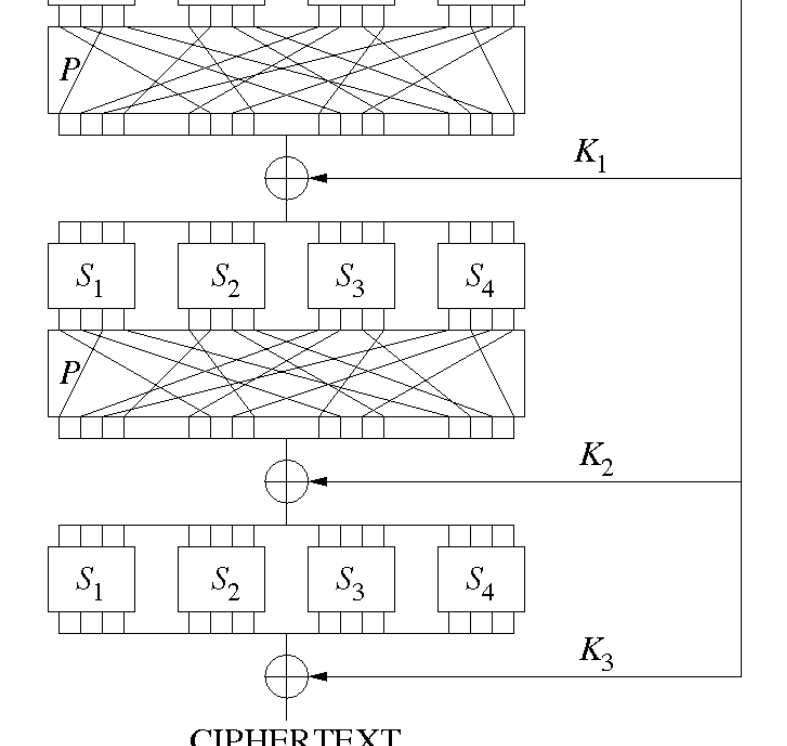
\includegraphics[width=86.10mm,height=204.93mm]{../../images/llm/page_064_img_01.png}%
\end{textblock*}

\end{document}
